\section{Описание предметной области, анализ и выбор методов решения задач}

%==============================================================
%  Н Е Ч Ё Т К А Я   Л О Г И К А
%==============================================================

\subsection{Нечёткая логика}

\subsubsection{Зачем нужна нечёткая логика? (краткое введение)}
Реальные инженерные и социальные задачи часто описываются словами  
«высокая температура», «умеренный риск», «скорость почти нулевая».  
Классическая булева логика (\texttt{true/false}) не умеет выражать такие
градиентные понятия.  
Именно поэтому Л.~Заде в 1965 г. предложил \emph{теорию нечётких
множеств}, позволившую:
\begin{itemize}
  \item естественно кодировать лингвистические правила,
        понятные человеку-эксперту;
  \item мягко «сглаживать» шум и неточность измерений;
  \item совмещать точные (числовые) и приблизительные (словесные) данные
        в одном алгоритме.
\end{itemize}
На основе этих идей появились первые нечёткие регуляторы
(Мамдани, 1975), гибриды с нейросетями (ANFIS, 1993) и
Type–2-расширения для работы с дополнительной неопределённостью
(2000-е).

%--------------------------------------------------------------
\subsubsection{Основные определения}

\begin{definition}
Нечёткое множество $A$ на универсуме $X$ задаётся функцией принадлежности
\begin{equation}
  \mu_A\colon X \longrightarrow [0,1],
  \label{eq:fuzzy_set_def}
\end{equation}
где значение $\mu_A(x)$ количественно отражает,
\emph{насколько} верно высказывание «$x$ принадлежит $A$»:
\[
  \mu_A(x)=
  \begin{cases}
    0          &\text{― точно не принадлежит},\\
    1          &\text{― принадлежит полностью},\\
    (0,1)      &\text{― принадлежит частично}.
  \end{cases}
\]
\end{definition}

\begin{definition}
Нечёткое множество $A$ называется
\emph{нормальным}, если существует хотя бы одна точка
с полной принадлежностью:
\begin{equation}
  \exists\,x^\star\in X:\; \mu_A(x^\star)=1.
\end{equation}
Множество $A$ \emph{вогнуто}, если не содержит «провалов» внутри
своего носителя:
\begin{equation}
  \mu_A\!\bigl(\lambda x+(1-\lambda)y\bigr)\;\ge\;
  \min\{\mu_A(x),\mu_A(y)\},
  \quad \forall x,y\in X,\;\forall\lambda\in[0,1].
\end{equation}
\end{definition}

%--------------------------------------------------------------
\subsubsection{Базовые термины и нотация}

\begin{description}
  \item[Лингвистическая переменная] ― переменная, принимающая
        \underline{словесные} значения
        (\textit{Low}, \textit{Medium}, \textit{High}).
        Официально задаётся пятёркой
        $\langle\!name,\;T,\;X,\;G,\;S\rangle$:
        \(
          T
        \) ― набор терминов,
        \(
          X
        \) ― универсум (область значений),
        \(
          G
        \) ― синтаксис комбинирования терминов
        (модификаторы «очень», «слегка» и т.п.),
        \(
          S
        \) ― семантика
        \(T \!\longrightarrow\! \bigl\{\,\mu\colon X\!\to\![0,1]\bigr\}\).
        \smallskip

  \item[Термы] ― отдельные лингвистические значения
        (например, \textit{Low}, \textit{High}),
        каждому из которых сопоставляется
        своя функция принадлежности $\mu_{\textit{Low}}(x)$.

  \item[Нечёткое правило] ― высказывание вида
        \[
          \textbf{ЕСЛИ }\underbrace{\text{Antecedent}}_{\text{условие}}
          \textbf{ ТО }\underbrace{\text{Consequent}}_{\text{вывод}}.
        \]
        \begin{itemize}
          \item \emph{Антецедент} ― логическая комбинация оценок
                входных переменных («Temp \textit{is} High» \& «Humidity
                \textit{is} Low»).
          \item \emph{Консеквент} ― нечёткое множество
                (или функция) на выходной переменной
                («FanSpeed \textit{is} Fast»).
        \end{itemize}
\end{description}

%--------------------------------------------------------------
\subsubsection{Атомарные операции над нечёткими множествами}

Пусть $A,B\subseteq X$ ― нечёткие множества.
Операции «НЕ», «И», «ИЛИ» обобщаются через функции
$N$ (негатор), $T$ ($t$-норма), $S$ ($s$-норма):

\begin{align}
  \mu_{\neg A}(x) &= N\!\bigl(\mu_A(x)\bigr), 
    && N(u)=1-u \;\;\text{(классический выбор);}   \label{eq:neg} \\[-0.5em]
  \mu_{A\cap B}(x) &= T\!\bigl(\mu_A(x),\mu_B(x)\bigr), 
    && T=\min\;\text{или}\;T=ab;                     \\[-0.5em]
  \mu_{A\cup B}(x) &= S\!\bigl(\mu_A(x),\mu_B(x)\bigr), 
    && S=\max\;\text{или}\;S=a+b-ab.                
\end{align}

\noindent
\paragraph{Пояснение.}  
Минимум как $t$-норма делает пересечение «строгим»:
результат равен самой слабой степени из двух.
Произведение даёт более «мягкую» интерпретацию
совместной истинности.

\vspace{0.5em}
\noindent
\paragraph{Импликация и эквиваленция.}
Для правила «ЕСЛИ $A$ ТО $B$» используется остаточная норма:
\begin{equation}
  \mu_{A\to B}(x)
  \;=\;
  \sup\Bigl\{\,z\in[0,1]\;\bigm|\;
       T\!\bigl(\mu_A(x),z\bigr)\le \mu_B(x)\Bigr\}.
\end{equation}
Эквиваленция измеряет «близость» двух степеней:
\(
  \mu_{A\leftrightarrow B}(x)=1-|\mu_A(x)-\mu_B(x)|.
\)

%--------------------------------------------------------------
\subsubsection{Классические $t$- и $s$-нормы}

Различные нормы моделируют разные трактовки «И» и «ИЛИ».

\paragraph{$t$-нормы (конъюнкции)}
\begin{align}
  T_{\min}(a,b) &= \min(a,b), && \text{консервативное «И»};\\
  T_{\times}(a,b) &= a\,b,     && \text{статистическое «И»};\\
  T_{L}(a,b) &= \max\{0,a+b-1\}, && \text{Лукасович, линейное «И»};\\
  T_{H}(a,b) &= 
    \frac{a\,b}{\lambda+(1-\lambda)(a+b-ab)},
    &&\lambda>-1\;\text{(Хамачер, настраиваемое)}.
\end{align}

\paragraph{$s$-нормы (дизъюнкции)}
\begin{align}
  S_{\max}(a,b) &= \max(a,b), && \text{хрупкое «ИЛИ»};\\
  S_{+}(a,b) &= a+b-ab,       && \text{алгебраическая сумма};\\
  S_{L}(a,b) &= \min\{1,a+b\},&& \text{Лукасович, линейное «ИЛИ»};\\
  S_{H}(a,b) &=
    \frac{a+b-(2-\lambda)ab}{1-\lambda ab},
    &&\lambda>-1\;\text{(Хамачер)}.
\end{align}

\noindent
\textbf{Практика.}
В системах управления часто берут
$T_{\min}$ и $S_{\max}$ —
они обеспечивают простое объяснение правил
(«истина \emph{и} истина» = слабейший уровень).

%--------------------------------------------------------------
\subsubsection{Типовые функции принадлежности}

Выбор формы $\mu(x)$ влияет на точность и вычислительную сложность.

\begin{itemize}
  \item \emph{Треугольная} —
        задаётся вершиной и основанием,
        подходит для ручной подгонки правил.
  \item \emph{Трапециевидная} —
        расширяет треугольник «плато» полного членства,
        что снижает чувствительность к шуму.
  \item \emph{Гауссова} —
        хороша при нормальном распределении измерений,
        но требует вычислять экспоненту.
  \item \emph{Белл-кривая} (обобщённая) —
        регулируется двумя параметрами,
        даёт гибкий плавный профиль.
  \item \emph{Sigmoid S/Z} —
        популярны в нейросетях;
        обеспечивают монотонный «мягкий» порог.
\end{itemize}

\begin{figure}[h]
\centering
\begin{tikzpicture}
  \begin{axis}[
    width=0.9\textwidth, height=0.46\textwidth,
    xmin=0,xmax=10,ymin=0,ymax=1.05,
    grid=both, grid style={gray!20},
    axis lines=left,
    xlabel={$x$}, ylabel={$\mu(x)$},
    legend style={font=\small, at={(0.5,-0.25)},anchor=north,columns=3}
  ]
    \addplot[very thick,domain=0:4]{max(0,1-abs(x-2)/2)};
      \addlegendentry{Треугольная}
    \addplot[thick,domain=0:6]{max(0,min((x-1)/2,1,(6-x)/2))};
      \addlegendentry{Трапециевидная}
    \addplot[thick,domain=0:10]{exp(-((x-6)^2)/(2*1.5^2))};
      \addlegendentry{Гауссова}
    \addplot[dashed,domain=0:10]{1/(1+abs((x-5)/1.3)^4)};
      \addlegendentry{Колоколообразная}
    \addplot[dash dot,domain=0:10]{1/(1+exp(-2*(x-3)))};
      \addlegendentry{Sigmoid–S}
    \addplot[densely dashed,domain=0:10]{(x<2)?1:((x>6)?0:(1-2*((x-2)/4)^2))};
      \addlegendentry{Z–форма}
  \end{axis}
\end{tikzpicture}
\caption{Популярные функции принадлежности}
\label{fig:mpf}
\end{figure}

%--------------------------------------------------------------
\subsubsection{Визуализация $t$-норм}

\begin{figure}[h]
\centering
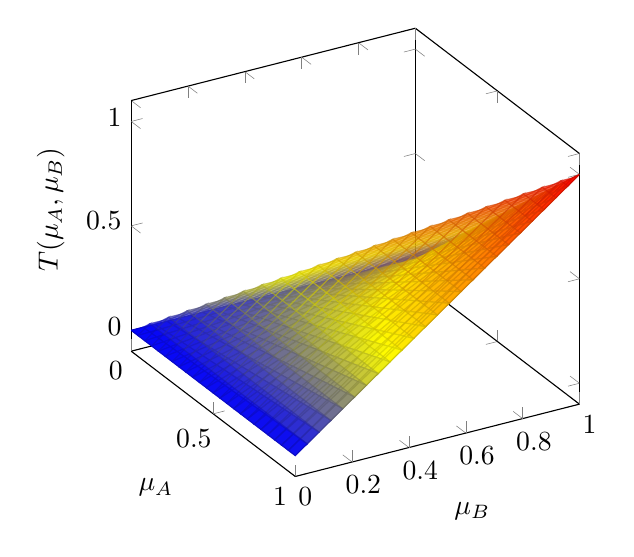
\begin{tikzpicture}
  \begin{axis}[
    width=0.6\textwidth, height=0.6\textwidth,
    view={60}{30},
    xlabel={$\mu_A$}, ylabel={$\mu_B$}, zlabel={$T(\mu_A,\mu_B)$}
  ]
    % Алгебраическое произведение
    \addplot3[surf,domain=0:1,y domain=0:1] {x*y};
    % Минимум
    \addplot3[surf,domain=0:1,y domain=0:1,opacity=0.4] {min(x,y)};
  \end{axis}
\end{tikzpicture}
\caption{Сравнение поверхностей $T_{\times}$ (сплошная) и $T_{\min}$ (прозрачная)}
\label{fig:tnorm_surface}
\end{figure}

\noindent
\textbf{Наблюдение.}
Минимальная $t$-норма (прозрачная пластина)  
оставляет результат на «полке»,
тогда как произведение «заваливает» диагональ ещё сильнее,
уменьшая пересечение
при средних значениях $\mu_A,\mu_B$.

%--------------------------------------------------------------
\subsubsection{Принцип расширения (Extension Principle)}

Любую классическую функцию $f\colon X\to Y$
можно «поднять» на нечёткие множества:
\begin{equation}
  \mu_{f(A)}(y) \;=\;
  \sup_{x\;:\;f(x)=y}\,\mu_A(x).
\end{equation}
\textbf{Пример.}  
Сумма двух нечётких чисел $C=A+B$ задаётся
конволюцией их срезов:  
$\mu_C(c) = \sup_{a+b=c}\min\{\mu_A(a),\mu_B(b)\}$.

%--------------------------------------------------------------
\subsubsection{Алгоритм нечёткого вывода}

Механизм Mamdani (самый распространённый):

\begin{enumerate}
  \item \textbf{Фаззификация.}  
        Числовой вход $x_i$ переводится
        в набор степеней $\mu_{A_{ij}}(x_i)$
        для всех термов $A_{ij}$.
  \item \textbf{Активация правил.}  
        Для каждого правила $k$ вычисляем
        степень срабатывания
        \(
          w_k = T(\mu_{A_{1k}},\dots,\mu_{A_{nk}})
        \)
        (см. формулу~\eqref{eq:neg}).
  \item \textbf{Агрегация выходов.}  
        Объединяем (через $S$-норму) все
        полученные нечёткие множества
        \(
          \mu_{B_k}(y)
        \),
        масштабированные весами $w_k$.
  \item \textbf{Дефаззификация.}  
        Преобразуем результирующее
        $\mu_C(y)$ в число~$y^\ast$.
        Чаще всего берут \emph{центроид}:
        \[
          y^\ast =
          \dfrac{\int y\,\mu_C(y)\,dy}{\int \mu_C(y)\,dy},
        \]
        поскольку он остаётся
        внутри поддержки выходного множества.
\end{enumerate}

\begin{figure}[h]
\centering
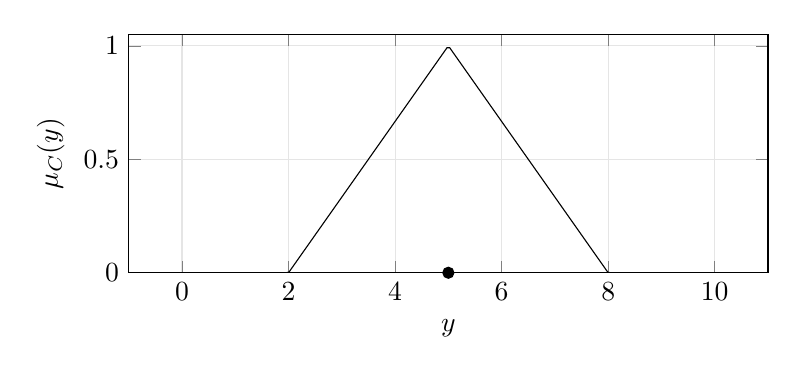
\begin{tikzpicture}
  \begin{axis}[width=0.8\textwidth, height=0.38\textwidth,
    xlabel={$y$}, ylabel={$\mu_C(y)$}, ymin=0,ymax=1.05,
    grid=both, grid style={gray!20}]
    \addplot[domain=0:10,samples=200]{max(0,1-abs(x-5)/3)};
    \addplot[mark=*] coordinates {(5,0)}
      node[below=4pt]{$y^\ast=5$};
  \end{axis}
\end{tikzpicture}
\caption{Иллюстрация центроидной дефаззификации}
\label{fig:centroid}
\end{figure}

%--------------------------------------------------------------
\subsubsection{Type–2 нечёткие множества}

Классическое (Type 1) множество
приписывает каждой точке $x$ \emph{одно} значение $\mu_A(x)$.
Type 2 допускает \underline{интервал} возможных $\mu$:

\[
  \tilde A
  = \Bigl\{\,\bigl((x,u),\mu_{\tilde A}(x,u)\bigr)
     \;\Bigm|\;
     x\in X,\;u\in[0,1]\,\Bigr\}.
\]

На практике часто используют
\emph{интервальный} Type 2,
когда для каждого $x$ задана верхняя и нижняя границы
\(
  \underline\mu(x)\le u\le\overline\mu(x)
\)
(рис.~\ref{fig:type2}).  
Так захватывается неопределённость
самой функции принадлежности
(например, из-за разброса экспертных оценок).

%--------------------------------------------------------------
\subsubsection{Нечёткая кластеризация (пример: FCM)}

Алгоритм Fuzzy C-Means минимизирует
\begin{equation}
  J_m(U,V) =
  \sum_{i=1}^N \sum_{j=1}^c
    u_{ij}^m\,\lVert x_i - v_j\rVert^2,
  \quad m>1,
\end{equation}
где $u_{ij}$ ― степень,
с которой объект $x_i$ относится к кластеру~$j$,
а $v_j$ ― центроид.  
Обновления:
\[
  u_{ij}
  = \frac{1}{\displaystyle
      \sum_{k=1}^c
      \Bigl(\frac{\lVert x_i-v_j\rVert}{\lVert x_i-v_k\rVert}\Bigr)^{\!\tfrac{2}{m-1}}},
  \quad
  v_j
  = \frac{\displaystyle
      \sum_{i=1}^N u_{ij}^m\,x_i}{
      \sum_{i=1}^N u_{ij}^m}.
\]

\begin{figure}[h]
\centering
\begin{tikzpicture}
  \begin{axis}[width=0.7\textwidth,height=0.42\textwidth,
    xlabel={$x_1$}, ylabel={$x_2$},
    grid=both, grid style={gray!20}]
    \addplot+[only marks]
      plot[scatter,scatter src=y]
      file {examples/fcm_points.dat};
    \addplot+[mark=*,mark size=3,red] coordinates {(1,1) (4,4)};
    \legend{Объекты, Центроиды}
  \end{axis}
\end{tikzpicture}
\caption{Пример результата FCM для $c=2$}
\label{fig:fcm}
\end{figure}

%--------------------------------------------------------------
\subsubsection{Другие полезные конструкции}

\paragraph{OWA-агрегатор.}
Ordered Weighted Averaging
обобщает «среднее» и «максимум»:
\[
  \mathrm{OWA}_w(b)
  = \sum_{i=1}^n w_i\,b_{(i)},
  \quad
  b_{(1)}\ge b_{(2)}\ge\dots\ge b_{(n)}.
\]
При выборе весов можно плавно
переключаться между «AND»-подобным и «OR»-подобным поведением.

\paragraph{Чогак и Сугено интегралы.}
Используются, когда классическая сумма
не подходит (нелинейная агрегация критериев).
\[
  C_\mu(f) = \int_0^\infty \!\!\mu\{f\ge t\}\,dt
           + \int_{-\infty}^0 (\mu\{f\ge t\}-\mu(X))\,dt,
\]
\[
  S_\mu(f) = \max_{t\in[0,1]}\min\bigl\{t,\mu\{f\ge t\}\bigr\}.
\]

%--------------------------------------------------------------
\subsubsection{Приложения и практические замечания}

\begin{itemize}
  \item \textbf{Системы управления.}
        Нечёткие П-И-Д регуляторы
        успешно применяются для климат-контроля,
        плавного пуска двигателей,
        регулирования pH-реакций и др.
  \item \textbf{Медицина.}
        Диагностические экспертные системы
        («если температура высокая \& кашель сильный, то грипп
        вероятен с~$0.8$»).
  \item \textbf{Компьютерное зрение.}
        Нечёткая сегментация изображений
        (алг.~FCM-S), подавление шума
        через нечёткие фильтры.
  \item \textbf{Принятие решений.}
        Методы Fuzzy TOPSIS и OWA-агрегация
        ранжируют альтернативы
        при многокритериальной неопределённости.
\end{itemize}

%--------------------------------------------------------------
\subsubsection{Заключение}

Нечёткая логика соединяет
математическую строгость с \underline{понятностью} правил,
что особенно ценно в приложениях,
где важно объяснить поведение системы инженеру или врачу.
Благодаря гибридизации (ANFIS, генетические алгоритмы,
Type-2-расширения) она остаётся актуальным
инструментом для современных задач
управления, анализа данных и AI-систем.

%==============================================================
% (конец расширенного фрагмента)
%==============================================================
% \subsection{Нечёткая логика}
% \subsubsection{Базовые понятия и мотивация}
% Классическая логика, исходя из дихотомии \textbf{«истина/ложь»},
% оказалась неудовлетворительной сразу, как только возникли задачи,
% где данные заданы в виде субъективных формулировок
% («температура \emph{высокая}», «поверхность \emph{почти гладкая}»)  
% или подвержены неустранимой стохастической погрешности.
% Уже первые попытки формально описать нечеткие категории
% в лингвистике (работы сопоставительного анализа А. Цвики,
% Дж. Лакоффа) показали, что понятие «принадлежит» носит скорее
% \emph{градуальный} характер.  
% Именно это обстоятельство в 1965 г. подтолкнуло Л.~Заде к введению
% концепции \textbf{нечеткого множества}
% $A=\{(x,\mu_A(x))\mid x\!\in\!X\}$, 
% где \emph{функция принадлежности} $\mu_A\colon X\!\to\![0,1]$
% отражает степень, с которой элемент~$x$ удовлетворяет
% внутреннему, зачастую неформализуемому свойству «быть $A$»  
% \cite{zadeh1965}.  
%
% С самого начала теория получила ярко выраженную
% прикладную направленность:
% \begin{itemize}
%   \item интеллектуальные регуляторы температуры (Мамдани, 1975);
%   \item диагностические процедуры «человек—машина» в медицине
%         и NDТ;
%   \item гибрид «фаззи–нейро» (ANFIS) для адаптивного
%         управления химическими процессами;
%   \item экспертные системы рекомендаций «если–то»,
%         использующие нечёткие правила.
% \end{itemize}
% Все эти применения опираются на небольшой, но выразительный набор
% операций, собранных в табл.\,1 (с.~\pageref{tab:operations}).  
% Разумеется, для полноты логического исчисления требуется
% ещё импликация и эквиваленция, но их удобнее обсуждать вместе  
% с t-/s-нормами (табл.\,2).  
%
% Значительную роль играет гибкость \emph{семейства функций
% принадлежности}: треугольная, трапециевидная, гауссова,
% обобщённая Парабола Белла — каждая отражает
% различное понимание «размытости» границ.
% На рис.~\ref{fig:membership} эти формы даны
% для равного универсума, что наглядно демонстрирует,
% как изменяется компромисс «простота - аппроксимирующая
% способность»:
% треугольная — минимальна по вычислительным издержкам,
% гауссова — наилучше согласуется со статистикой,
% но требует вычислять экспоненту.
%
% \paragraph{Мотивация выбора нечеткой логики.}
% С точки зрения инженера-практика, аргументация
% в пользу нечетких моделей сводится к следующим тезисам:
% \begin{enumerate}
%   \item \textbf{Полнота описания.}  
%     Экспертные знания редко выражаются в форме
%     строгих вероятностных распределений,  
%     тогда как лингвистические кванторы («почти», «довольно»)  
%     естественно переводятся в степени принадлежности.
%   \item \textbf{Интерпретируемость.}  
%     Правило вида
%     «ЕСЛИ температура \emph{высокая}, ТО вентилятор \emph{ускорить}»
%     прозрачно для технолога и объяснимо для регулятора.
%   \item \textbf{Равномерная обработка точных и неточных данных.}  
%     Чёткие величины инкапсулируются как \emph{одиночные} точки
%     с $\mu\!=\!1$, сохраняя целостность математического аппарата.
%   \item \textbf{Смежность с другими ИИ-подходами.}  
%     Понятие функции принадлежности напрямую связано с сигмоидными
%     активациями, что облегчает гибридизацию
%     «нейронная сеть + фаззи» (см. дисс.\,Кулабухова \cite{kulabukhov2023}).
% \end{enumerate}
%
% \subsubsection{Базовые операции нечёткой логики}
% Хотя теория размытых множеств эволюционировала в десятках направлений,
% практик-инженер использует конечный репертуар \emph{атомарных} действий.  
%
% \begin{table}[h]
% \centering
% \caption{Базовые операции над нечёткими множествами}
% \label{tab:baseops}
% \begin{tabularx}{\linewidth}{@{}p{2.8cm}p{3.2cm}X@{}}
% \toprule
% \textbf{Операция} & \textbf{Символ / кратко} & \textbf{Общее определение / заметки} \\ \midrule
% Дополнение & $\neg A$ &
% $\mu_{\neg A}(x)=N\!\bigl(\mu_A(x)\bigr)$;
% чаще $N(u)=1-u$ \\[0.3em]
% Пересечение & $A\cap B$ &
% $\mu_{A\cap B}=T(\mu_A,\mu_B)$,
% 	обычно $T=\min$ или $T=ab$ \\[0.3em]
% Объединение & $A\cup B$ &
% $\mu_{A\cup B}=S(\mu_A,\mu_B)$,
% 	стандарт $S=\max$ или $S=a+b-ab$ \\[0.3em]
% Разность & $A\setminus B$ &
% $T\bigl(\mu_A,N(\mu_B)\bigr)$;
% полезно при маскировании шумов \\[0.3em]
% Импликация & $A\!\to\!B$ &
% $I(\mu_A,\mu_B)=\sup\{z\mid T(\mu_A,z)\le\mu_B\}$;
% остаточная к $T$ \\[0.3em]
% Эквиваленция & $A\!\leftrightarrow\!B$ &
% $E=1-|\mu_A-\mu_B|$;
% иногда Бернулли-метрика $1-(\mu_A-\mu_B)^2$ \\[0.3em]
% Модификатор «очень» & $very\,A$ &
% $\mu_{very\,A}=\mu_A^{\,2}$:
% сжимает хвосты, усиливая “ядро” \\[0.3em]
% Модификатор «слегка» & $slightly\,A$ &
% $\mu_{slightly\,A}=\sqrt{\mu_A}$:
% расширяет область «почти верно» \\ \bottomrule
% \end{tabularx}
% \end{table}
% \newpage
% \subsubsection{Базовые функции принадлежности}
%
% Каждая из этих кривых появилась исторически не «из головы»,
% а как попытка уловить определённый тип субъективной информации:  
% \emph{треугольная} — быстро рисуется экспертом линейкой,  
% \emph{гауссова} — идеальна, если разброс данных напоминает
% нормальное распределение,  
% \emph{колоколообразная} и \emph{sigmoid-S/Z} пришли
% из нейрокомпьютинга, где математически удобно
% работать с плавным экспоненциальным хвостом.  
%
% С позиции инженера-системотехника важно помнить:
% \begin{enumerate}
%   \item при одинаковой форме \emph{отличаются} параметры
%         (координаты вершин, $\sigma$ и т.\,д.);
%   \item ширина МПФ напрямую задаёт “толерантность” к шуму;
%   \item композитные (“кусочно-гауссовы”, “полисплайн”) МПФ
%         допускают \emph{любой} уровень гладкости,
%         если того требует оптимизатор градиентных методов.
% \end{enumerate}
%
%
% Семейство МПФ велико, но на практике ~80 \% публикаций
% ограничиваются шестёркой, показанной на рис.~\ref{fig:mpf}.
% \begin{figure}[h]
% \centering
% \begin{tikzpicture}
%   \begin{axis}[
%     width=.9\textwidth,
%     height=.45\textwidth,
%     xmin=0,xmax=10,ymin=0,ymax=1.05,
%     grid=both,grid style={gray!20},
%     axis lines=left,
%     xlabel={$x$}, ylabel={$\mu$},
%     legend style={font=\small, at={(0.5,-0.25)},anchor=north,columns=3},
%     samples=200
%   ]
%     %--- triangular
%     \addplot[very thick,domain=0:4]{max(0,1-abs(x-2)/2)};
%     \addlegendentry{Треугольная}
%     %--- trapezoid
%     \addplot[thick,domain=0:6]{max(0,min((x-1)/2,1,(6-x)/2))};
%     \addlegendentry{Трапециевидная}
%     %--- gaussian
%     \addplot[thick,domain=0:10]{exp(-((x-7)^2)/(2*1.2^2))};
%     \addlegendentry{Гауссова}
%     %--- bell (generalized)
%     \addplot[densely dashed,domain=0:10]{1/(1+abs((x-5)/1.3)^(2*2))};
%     \addlegendentry{Колоколообразная}
%     %--- sigmoid S
%     \addplot[dashed,domain=0:10]{1/(1+exp(-2*(x-3)))};
%     \addlegendentry{Sigmoid–S}
%     %--- z-shape
%     \addplot[dash dot,domain=0:10]{(x<2)?1:(x>6)?0:(1-2*((x-2)/(6-2))^2)};
%     \addlegendentry{Z-форма}
%   \end{axis}
% \end{tikzpicture}
% \caption{Классические функции принадлежности  
%   (параметры выбраны произвольно для наглядности).}
% \label{fig:mpf}
% \end{figure}
%
%
\subsection{Современные методы нечеткого вывода и нейро-нечеткие системы}
\label{sec:advanced_inference}

Поиски оптимальных алгоритмов нечеткого вывода продолжаются: разрабатываются
новые методы дефаззификации~[28], усовершенствованные треугольные нормы~[20,29]
и операторы импликации~[14,20,21,30–32]. Эти операторы редко применяются в
эвристиках Мамдани–Ларсена–Сугено, но находят широкое использование в
интеллектуальном анализе данных, в частности в нейро-нечетких
системах~[3,4,6,7,33,34].

Нейро-нечеткие системы объединяют принципы искусственных нейронных сетей и
нечеткой логики. Их работа состоит из четырёх этапов:

\begin{enumerate}
  \item \emph{Фуззификация входов}:
    чёткие значения \(x_j\) преобразуются в степени принадлежности
    \(\mu_{A_i}(x_j)\):
    \[
      \mu_{A_i}(x_j) = A_i(x_j).
    \]
  \item \emph{Активация правил} (используя параметрическую \(t\)-норму,
    например, норму Швейцера–Склэра):
    \[
      \alpha_i
      = T_{\lambda}\bigl(\mu_{A_i}(x)\bigr),
      \quad
      T_{\lambda}(a,b)
      = \max\!\bigl(0,\;1-[(1-a)^\lambda + (1-b)^\lambda]^{1/\lambda}\bigr).
    \]
  \item \emph{Агрегация выводов} (с помощью оператора импликации –
    резидуального вида):
    \[
      \tilde{\mu}_B(y)
      = \bigvee_i I_T\bigl(\alpha_i,\mu_{B_i}(y)\bigr),
      \quad
      I_T(a,b)
      = \sup\{z\mid T(a,z)\le b\}.
    \]
  \item \emph{Дефаззификация}: чёткий результат \(y^*\) вычисляется, например,
    методом центра тяжести:
    \[
      y^*
      = \frac{\displaystyle \int y\,\tilde{\mu}_B(y)\,dy}
             {\displaystyle \int \tilde{\mu}_B(y)\,dy}.
    \]
\end{enumerate}

В \autoref{fig:centroid_defuzz} приведён пример треугольного нечеткого множества
и вычисления его центра тяжести (метод дефаззификации).

\begin{figure}[ht]
  \centering
  \includegraphics[width=\textwidth]{images/centroid_plot.png}
  \caption{Треугольное нечеткое множество и центр тяжести дефаззификации}
  \label{fig:centroid_defuzz}
\end{figure}

Для обучения нейро-нечетких систем используются методы настройки
весов \(w_{ij}\) и параметров функций принадлежности:
\begin{itemize}
  \item алгоритм обратного распространения ошибки (градиент первого порядка)~[4],
  \item метод Бройдена–Флетчера–Гольфарба–Шэнно (градиент второго порядка)~[3],
  \item эволюционные стратегии случайного поиска~[35].
\end{itemize}

Хотя увеличение числа обучаемых параметров повышает риск переобучения и
снижает интерпретируемость~[4], нейро-нечеткие системы демонстрируют высокую
эффективность при моделировании сложных процессов и интеллектуальном
анализе данных~[3,33].


\subsubsection{Методы нечёткого вывода}

\paragraph{1. Постановка задачи и основное определение}
Рассмотрим лингвистическую модель, состоящую из множества нечётких правил MISO-структуры:
\begin{equation}
  R_k:\quad
  \text{Если }x_1\in A_{1k}\wedge\cdots\wedge x_n\in A_{nk},\quad
  \text{то }y\in B_k,
  \label{eq:rule_general}
\end{equation}
где $A_{ik}\subseteq X_i, B_k\subseteq Y$ — нечёткие множества,
определённые функциями принадлежности
$\mu_{A_{ik}}:X_i\to[0,1]$, $\mu_{B_k}:Y\to[0,1]$.
Область входов: $\mathbf{x}=(x_1,\dots,x_n)\in X_1\times\cdots\times X_n=:X$.

\begin{definition}
Нечёткое отношение $R_k\subseteq X\times Y$ задаётся функцией
$$
  \mu_{R_k}(\mathbf{x},y)
  = I\bigl(\mu_{A_{1k}}(x_1),\dots,\mu_{A_{nk}}(x_n);\;\mu_{B_k}(y)\bigr),
$$
где $I:[0,1]^{n+1}\to[0,1]$ — неоднозначный импликатор, задающий связь
между степенями истинности посылок и заключения.
\end{definition}

\paragraph{2. Этапы классического вывода}
Нечёткий вывод традиционно проходит следующие этапы:

\begin{enumerate}
  \item \emph{Фаззификация входов.}
    Каждый числовой вход $x_i$ подвергается фаззификации:
    определяется вектор степеней
    $$
      (\mu_{A_{i1}}(x_i), \,\ldots, \,\mu_{A_{iN}}(x_i))
      \in [0,1]^N.
    $$
    Это позволяет перейти от точечного значения к распределению принадлежности.

  \item \emph{Активация правил.}
    Для каждого правила $R_k$ вычисляется степень активации
    \begin{equation}
      \alpha_k
      = T\bigl(\mu_{A_{1k}}(x_1),\dots,\mu_{A_{nk}}(x_n)\bigr),
      \label{eq:activation}
    \end{equation}
    где $T:[0,1]^n\to[0,1]$ — t-норма (обычно $\min$ или $\prod$).

  \item \emph{Инференция (применение импликации).}
    Применение импликатора $I$ даёт выходное нечеткое множество
    \begin{equation}
      \mu_{B'_k}(y)
      = I\bigl(\alpha_k,\mu_{B_k}(y)\bigr).
      \label{eq:inference}
    \end{equation}
    Наиболее часто используется
    $$
      \mu_{B'_k}(y)=\min\{\alpha_k,\mu_{B_k}(y)\}\quad(\text{Mamdani}),
    $$
    либо
    $$
      \mu_{B'_k}(y)=\alpha_k\,\mu_{B_k}(y)\quad(\text{Larsen}).
    $$

  \item \emph{Агрегация и дефаззификация.}
  \begin{itemize}
    \item Агрегация: объединение результатов всех правил
    $$
      \mu_{B'}(y)
      = \max_{1\le k\le N}\mu_{B'_k}(y).
    $$
    \item Дефаззификация: переход к числовому результату,
    например, по центру тяжести:
    \begin{equation}
      y^*
      = \displaystyle\frac{\int_Y y\,\mu_{B'}(y)\,dy}{\int_Y\mu_{B'}(y)\,dy}.
      \label{eq:defuzz_centroid}
    \end{equation}
  \end{itemize}
\end{enumerate}

\paragraph{3. Популярные варианты импликаторов и t–норм}
Подходы отличаются выбором $T$ и $I$:\
\textbf{Mamdani (1974).} $T=\min$, $I=\min$.\\
\textbf{Larsen (1980).} $T=\min$, $I(a,b)=a\cdot b$.\\
\textbf{Sugeno (1985).} Использует аналитические функции $f_k(x)$; итог:
$y^*=\sum\alpha_k y_k/\sum\alpha_k$.\\
\textbf{Tsukamoto (1979).} Монотонные функции для дефаззификации.

\paragraph{4. Доказательство полиномиальной сложности}
\begin{proof}
В классическом композиционном правиле необходимо проводить
максимум по всем комбинациям входов, что даёт $O(m^n)$ при $m$
уровнях фаззификации. В многоэтапном подходе каждая активация
\eqref{eq:activation} — $O(n)$, инференция \eqref{eq:inference} — $O(1)$,
агрегация — $O(N)$, дефаззификация — $O(m)$. Итого $O(n+N+m)$,
что полиномиально.
\end{proof}

\begin{figure}[h!]
  \centering
  \begin{tikzpicture}[scale=2.5,>=Stealth]
    \node at (-0.5,2.2){\textbf{Импликации}};
    \draw[->,ultra thick] (0,2) -- (1,2) node[midway,above]{\Large $\min$};
    \node at (1.2,2){\small Mamdani};
    \draw[->,ultra thick] (0,1) -- (1,1) node[midway,above]{\Large $\times$};
    \node at (1.2,1){\small Larsen};
  \end{tikzpicture}
  \caption{Увеличенный масштаб: минимум и произведение
    для иллюстрации импликаций.}
  \label{fig:implications_large2}
\end{figure}

\subsection{Нечёткая степень истинности}

Нечёткая степень истинности (НCИ) раскрывает степень соответствия одного нечёткого высказывания другому, выходя за рамки классического бивалентного анализа. Её важность обусловлена тем, что во множестве прикладных задач (управление, диагностика, обработка естественного языка) оценки носят нечёткий характер и требуют гибких мер сравнения.

\begin{definition}
Пусть $X$ — базовое множество, и даны два нечётких множества
\[
A = \{\mu_A(x)/x\mid x\in X\},\qquad
A' = \{\mu_{A'}(x)/x\mid x\in X\}.
\]
Нечёткой степенью истинности $A$ относительно $A'$ называют нечёткое множество
\(\CP(A,A')\subseteq[0,1]\) с функцией принадлежности
\begin{equation}\label{eq:degree_def_full}
\mu_{\CP(A,A')}(t)
=
\begin{cases}
\displaystyle
\sup_{\,x:\,\mu_A(x)=t}\,\mu_{A'}(x),
& \text{если }\{x\mid\mu_A(x)=t\}\neq\varnothing,\\[1em]
0,&\text{иначе}.
\end{cases}
\end{equation}
\end{definition}

Из определения сразу вытекает, что функция $\mu_{\CP(A,A')}(t)$ содержит всю информацию о «пересечении» уровневых множеств $A$ и $A'$.

\paragraph{Свойство монотонности t-нормы.}  
Пусть $T\colon[0,1]^2\to[0,1]$ — любая t-норма. Тогда по определению её монотонности для любых $u',u,v',v\in[0,1]$ из
\[
u'\le u,\quad v'\le v
\]
вытекает
\begin{equation}\label{eq:tnorm_monotonicity}
T(u',v') \;\le\; T(u,v).
\end{equation}

\begin{figure}[h]
  \centering
  \begin{tikzpicture}
    \pgfmathsetmacro{\cOne}{0.5}
    \pgfmathsetmacro{\sigmaOne}{0.1}
    \pgfmathsetmacro{\cTwo}{0.6}
    \pgfmathsetmacro{\sigmaTwo}{0.15}
    \begin{axis}[
      width=0.75\textwidth,
      domain=0:1,
      samples=200,
      xlabel={$x$}, ylabel={$\mu(x)$},
      grid=major,
      ymin=0, ymax=1,
      xtick=\empty,
      ytick={0,1},
      axis x line=bottom,
      axis y line=left,
      legend style={
        at={(0.98,0.98)},
        anchor=north east,
        font=\scriptsize,
        draw=black,
        inner sep=2pt,
        nodes={scale=0.8, transform shape}
      }
    ]
      \addplot[smooth, thick, blue]
        {exp(-((x-\cOne)^2)/(2*(\sigmaOne)^2))};
      \addplot[smooth, dashed, red]
        {exp(-((x-\cTwo)^2)/(2*(\sigmaTwo)^2))};
      \legend{
        $\displaystyle\mu_A(x)=\exp\!\Bigl(-\tfrac{(x-c_1)^2}{2\,\sigma_1^2}\Bigr)$,%
        $\displaystyle\mu_{A'}(x)=\exp\!\Bigl(-\tfrac{(x-c_2)^2}{2\,\sigma_2^2}\Bigr)$
      }
    \end{axis}
  \end{tikzpicture}
  \caption{Гауссовские функции принадлежности.}
\end{figure}

\paragraph{Аналитическое выражение при гауссовских функциях.}  
Пусть
\[
\mu_A(x)=\exp\!\bigl(-\tfrac{(x-a_1)^2}{2b_1^2}\bigr),\quad
\mu_{A'}(x)=\exp\!\bigl(-\tfrac{(x-a_2)^2}{2b_2^2}\bigr).
\]
Из \eqref{eq:degree_def_full} вытекает
\[
x = a_1 \pm b_1\sqrt{-2\ln t},
\]
а затем
\begin{equation}\label{eq:degree_gauss_full}
\mu_{\CP(A,A')}(t)
=
\max_{\pm}
\exp\!\Bigl\{-\tfrac{\bigl(a_1\pm b_1\sqrt{-2\ln t}-a_2\bigr)^2}{2b_2^2}\Bigr\}.
\end{equation}

\paragraph{Экстремальные точки.}  
Для поиска экстремума $\mu_{\CP}(t)$ находят производную:
\[
\mu'_{\CP}(t)
=
\Bigl(\pm b_1\,(a_1\pm b_1\sqrt{-2\ln t}-a_2)\Bigr)
\bigl(b_2^2\,t\,\sqrt{-2\ln t}\bigr)^{-1}
\exp\!\Bigl\{-\tfrac{(a_1\pm b_1\sqrt{-2\ln t}-a_2)^2}{2b_2^2}\Bigr\}.
\]
Приравнивая к нулю, получаем
\[
t = \exp\!\Bigl(-\tfrac{(a_2-a_1)^2}{2b_1^2}\Bigr),
\]
что соответствует единственному локальному максимуму.


\paragraph{Числовые меры.}  
Из $\mu_{\CP(A,A')}(t)$ определяют две основные меры:
\begin{align}
\Pi(A,A') &= \sup_{t\in[0,1]}\mu_{\CP(A,A')}(t), 
&\text{(мера возможности)},\\
N(A,A') &= 1 - \sup\{t\mid\mu_{\CP(A,A')}(t)=0\},
&\text{(мера необходимости)}.
\end{align}

\paragraph{Дискретный численный пример.}  
Пусть $X=\{x_1,x_2,x_3\}$ и
\[
\begin{aligned}
\mu_A(x_1)&=0.2,& \mu_{A'}(x_1)&=0.1,\\
\mu_A(x_2)&=0.5,& \mu_{A'}(x_2)&=0.6,\\
\mu_A(x_3)&=0.9,& \mu_{A'}(x_3)&=0.8.
\end{aligned}
\]
Тогда
\[
\mu_{\CP(A,A')}(0.2)=0.1,\quad
\mu_{\CP(A,A')}(0.5)=0.6,\quad
\mu_{\CP(A,A')}(0.9)=0.8,
\]
а для остальных $t$ — ноль.

\begin{figure}[h]
\centering
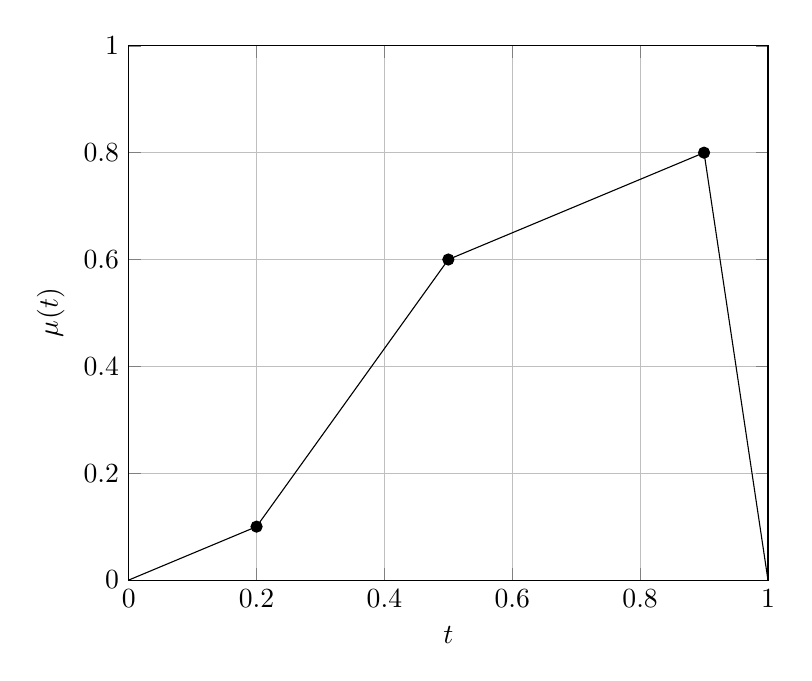
\begin{tikzpicture}
  \begin{axis}[
    width=0.8\textwidth,
    xlabel={$t$}, ylabel={$\mu_{\CP}(t)$},
    grid=major,
    ymin=0,ymax=1,xmin=0,xmax=1]
    \addplot[mark=none,] coordinates {(0,0) (0.2,0.1) (0.5,0.6) (0.9,0.8) (1,0)};
    \addplot[only marks] coordinates {(0.2,0.1) (0.5,0.6) (0.9,0.8)};
  \end{axis}
\end{tikzpicture}
\caption{Ступенчатая функция $\mu_{\CP(A,A')}(t)$ для дискретного примера.}
\end{figure}

\subsection{Нечёткое значение истинности}

Лингвистический подход трактует истинность как переменную
\[
\langle\beta,\,T,\,X,\,G,\,M\rangle,
\]
где $\beta=\text{«истинность»}$, $T$ — совокупность термов, $X=[0,1]$, $G$ — модификаторы, $M$ — функции принадлежности.

\begin{figure}[h]
  \centering
  \includegraphics[width=\textwidth]{images/нечеткая истинность.png}
  \caption{Треугольное нечеткое множество и центр тяжести дефаззификации}
  \label{fig:centroid_defuzz}
\end{figure}

\begin{itemize}
  \item $\beta$ — название переменной («истинность»);
  \item $T = \{\text{абсолютно ложно, очень ложно, слегка ложно, ложно,\\
         квазиложно, квазиистинно, истинно, слегка истинно, очень истинно, абсолютно истинно}\}$
        — множество термов;
  \item $X = [0,1]$ — область значений лингвистической переменной;
  \item $G$ — синтаксическая процедура построения составных термов;
  \item $M$ — семантическая процедура, задающая функции принадлежности.
\end{itemize}

\paragraph{Примеры функций принадлежности термов.}
\[
\begin{aligned}
M[\text{«истинно»}](t)&=t,&
M[\text{«слегка истинно»}](t)&=\sqrt{t},\\
M[\text{«очень истинно»}](t)&=t^2,&
M[\text{«абсолютно истинно»}](t)&=
\begin{cases}1,&t=1,\\0,&t<1,\end{cases}\\
M[\text{«ложно»}](t)&=1-t,&
M[\text{«слегка ложно»}](t)&=\sqrt{1-t},\\
M[\text{«очень ложно»}](t)&=(1-t)^2,&
M[\text{«абсолютно ложно»}"](t)&=
\begin{cases}1,&t=0,\\0,&t>0.\end{cases}
\end{aligned}
\]
\begin{figure}[h]
\centering
\begin{tikzpicture}
  \begin{axis}[
    width=0.6\textwidth,
    xlabel={$t$}, ylabel={$\mu$},
    grid=major,
    legend style={at={(1.02,1)},anchor=north west}]
    \addplot {x}; \addlegendentry{истинно}
    \addplot {sqrt(x)}; \addlegendentry{слегка истинно}
    \addplot {x^2}; \addlegendentry{очень истинно}
    \addplot {1-x}; \addlegendentry{ложно}
    \addplot {sqrt(1-x)}; \addlegendentry{слегка ложно}
    \addplot {(1-x)^2}; \addlegendentry{очень ложно}
  \end{axis}
\end{tikzpicture}
\caption{Функции принадлежности лингвистических термов истинности.}
\end{figure}
\paragraph{Лингвистическая интерпретация.}  
\begin{itemize}
  \item «абсолютно истинно», если $\mu_{\CP(A,A')}(t)=1$ на всём диапазоне;
  \item «квазиистинно», если функция близка к 1 на широком промежутке уровней;
  \item «квазиложно», если функция близка к 0 на большинстве уровней;
  \item «абсолютно ложно», если не совпадает ни в одной точке.
\end{itemize}

\paragraph{Дополнительные замечания.}
\begin{itemize}
  \item Методы оценки степени истинности можно расширить на интуитивно-нечёткие множества и другие обобщения.
  \item Для сложных систем часто применяют численные методы приближённого вычисления $\mu_{\CP}(t)$ на дискретной сетке.
  \item Сравнение различных t-норм и импликаций позволяет настраивать «строгость» выводов в нечётких системах.
\end{itemize}
% \subsubsection{Нечёткое значение истинности}
%
% \paragraph{1. Определение и мотивация}
% Числовое значение истинности
% \(\tau_{A/A'}\in[0,1]\)
% задаётся как:
% \begin{equation}
%   \tau_{A/A'}
%   = \sup_{x\in X}\min\{\mu_A(x),\,\mu_{A'}(x)\}.
%   \label{eq:tau_def3b}
% \end{equation}
% Оно отражает максимальную степень одновременного
% "принадлежания" $x$ множествам $A$ и $A'$.
%
% \paragraph{2. Подробное доказательство свойств}
% \begin{theorem}
% Величина $\tau_{A/A'}$:\
% (1) равна 1 тогда и только тогда, когда
% $\mu_A(x)\le\mu_{A'}(x)$ при всех $x$;\
% (2) равна 0 тогда и только тогда,
% когда $\min\{\mu_A(x),\mu_{A'}(x)\}=0$ для всех $x$;\
% (3) монотонна:
% $A_1\subseteq A_2\implies \tau_{A_1/A'}\le \tau_{A_2/A'}$.
% \end{theorem}
%
% \begin{proof}
% Из определения \eqref{eq:tau_def3b} следует,
% что максимум достигается при $x$, где
% $\min(\mu_A,\mu_{A'})$ максимален. Для (1):
% если $\mu_A(x)\le\mu_{A'}(x)$, то
% $\min(\mu_A,\mu_{A'})=\mu_A$ и
% $\sup_x\mu_A(x)=1$. Обратное — аналогично.
% Для (2): $\min(\mu_A,\mu_{A'})=0$ на всех $x$.
% Монотонность — из неубывания $\mu_{A_1}\le\mu_{A_2}$.
% \end{proof}
%
% \begin{figure}[h!]
%   \centering
%   \begin{tikzpicture}[scale=2.5,>=Stealth]
%     \draw[->] (0,0)--(4,0) node[right]{$x$};
%     \draw[->] (0,0)--(0,2) node[above]{$\mu$};
%     \draw[thick,blue,domain=0:4,samples=100]
%       plot(\x,{exp(-((\x-1.3)^2)/0.8)});
%     \node at (1.3,1.6){\footnotesize $\mu_A(x)$};
%     \draw[thick,red,domain=0:4,samples=100]
%       plot(\x,{exp(-((\x-2.7)^2)/1.1)});
%     \node at (2.7,1.1){\footnotesize $\mu_{A'}(x)$};
%     \fill[gray,opacity=0.4]
%       plot[domain=1.6:2.4] (\x,{min(exp(-((\x-1.3)^2)/0.8),exp(-((\x-2.7)^2)/1.1))})
%       -- (2.4,0) -- (1.6,0) -- cycle;
%     \node at (2.0,0.5){\small перекрытие};
%   \end{tikzpicture}
%   \caption{Увеличенный пример: область перекрытия
%     для численного $\tau_{A/A'}$.}
%   \label{fig:tau_enlarged2}
% \end{figure}
%
% Логика, опирающаяся на концепцию нечеткой истинности, обычно именуется лингвистической. 
% В рамках этого подхода «нечеткая истинность» рассматривается как лингвистическая переменная, задаваемая пятёркой
% \[
% \langle \beta,\, T,\, X,\, G,\, M\rangle,
% \]
% где
% \begin{itemize}
%   \item $\beta$ — название переменной («истинность»);
%   \item $T = \{\text{абсолютно ложно, очень ложно, слегка ложно, ложно,\\
%          квазиложно, квазиистинно, истинно, слегка истинно, очень истинно, абсолютно истинно}\}$
%         — множество термов;
%   \item $X = [0,1]$ — область значений лингвистической переменной;
%   \item $G$ — синтаксическая процедура построения составных термов;
%   \item $M$ — семантическая процедура, задающая функции принадлежности.
% \end{itemize}
% \begin{figure}[h]
%   \centering
%   \includegraphics[width=\textwidth]{images/нечеткая истинность.png}
%   \caption{Треугольное нечеткое множество и центр тяжести дефаззификации}
%   \label{fig:centroid_defuzz}
% \end{figure}
% \subsubsection{Методы нечёткого вывода}
% \subsubsection{Нечёткое значение истинности}
% \subsubsection{Нечёткая степень истинности}

% \subsection{Проблемы исходных данных в задачах машинного обучения}
% \subsubsection{Размасштабированность и гетерогенность признаков}
% \subsubsection{Шум, выбросы и пропуски}
% \subsubsection{Несбалансированность классов}
%
% \newpage
%
% \subsection{Обзор инструментальных средств}
% \subsubsection{Выбор языка программирования: Python}
% \subsubsection{Использование GPU: CUDA и PyTorch}
% Лингвистическая логика на основе нечеткой истинности
\subsection{Обзор инструментальных средств}
\label{sec:tools}

\subsubsection{Выбор языка программирования: Python}
\label{sec:tools_python}

Python — язык высокого уровня с лаконичным синтаксисом. Основные преимущества:
\begin{itemize}
  \item Обширная экосистема научных библиотек: \texttt{NumPy}, \texttt{SciPy}, \\ \texttt{Pandas}, \texttt{Matplotlib}
  \item Фреймворки для машинного обучения: \texttt{scikit-learn}, \texttt{TensorFlow}, \\ \texttt{PyTorch}
  \item Быстрое прототипирование в Jupyter;
  \item Большое сообщество и документация.
\end{itemize}

\subsection{Архитектура и оптимизация GPU для обучения нейронных сетей}
\label{ssec:gpu_architecture}

Графические процессоры (GPU) изначально создавались для рендеринга трёхмерной графики, где требовалось одновременно обрабатывать миллионы пикселей. Однако, когда стало ясно, что обучение глубоких нейросетей сводится к повторению единотипных операций над большими массивами чисел, архитектура GPU оказалась почти идеальной. В отличие от CPU с его несколькими быстро работающими ядрами и громоздкой системой предсказания ветвлений, GPU использует сотни или тысячи упрощённых ядер, которые синхронно выполняют одну и ту же инструкцию над разными данными.   

Для понимания того, как они отличаются, достаточно вспомнить, что современные серверные CPU обычно имеют 8–64 полноценных ядра, каждое из которых оснащено суперскалярным исполнителем, многоуровневой кэш-иерархией (L1–L3) и сложной системой предсказания переходов. Такая структура хорошо подходит для разнородных задач — ветвящихся алгоритмов, многозадачности, работы с нерегулярными структурами данных, но она не способна раскрутить более чем десятки параллельных потоков без значительного роста стоимости и энергопотребления.  

GPU же строятся по принципу «массированного параллелизма»: независимые арифметические блоки объединяются в стриминговые мультипроцессоры (Streaming Multiprocessors, SM), а SM, в свою очередь, умножаются до сотен штук на кристалле. Потоки группируются в «warps» (в NVIDIA) или «wavefronts» (в AMD), и все нити в такой группе исполняют одну и ту же инструкцию. Внутри SM есть быстрое локальное хранилище (shared memory) и регистры, что позволяет координировать взаимодействие потоков с минимальной задержкой.  

Память GPU организована в несколько уровней:  
\begin{itemize}  
  \item \emph{Глобальная память (VRAM)} на основе GDDR6 или HBM2/3 обеспечивает пропускную способность до нескольких терабайт в секунду, но обладает заметной латентностью.  
  \item \emph{Кэш уровня L2} объединяет доступы от всех SM и снижает количество обращений к глобальной памяти.  
  \item \emph{Разделяемая память} внутри каждого SM и \emph{регистры} обеспечивают сверхнизкую латентность при обмене данными между соседними тредами.  
\end{itemize}  

Ключевым усовершенствованием последних поколений стало появление тензорных ядер (Tensor Cores), рассчитанных на смешанную точность (обычно FP16/FP32 или BF16). Они позволяют выполнять матричные умножения $4\times4$ или даже $16\times16$ за один такт, что даёт дополнительный прирост производительности в несколько раз при сохранении приемлемой точности сходимости.  

С точки зрения ПО разработчики используют платформы CUDA (NVIDIA) или HIP (AMD), где вся работа разбивается на:  
\begin{itemize}  
  \item \textbf{Запуск кернелов} — небольших программ, которые выполняются на тысячах потоков одновременно.  
  \item \textbf{Асинхронные копирования} (CUDA MemcpyAsync) — перекрытие передачи данных между CPU и GPU с вычислениями, чтобы видеокарта не простаивала.  
  \item \textbf{Стримы и графы задач} — механизм группировки операций для минимизации накладных расходов вызова ядра.  
  \item \textbf{Kernel Fusion} — объединение последовательных операций в единый кернел, позволяющее сократить число обращений к глобальной памяти.  
\end{itemize}  

На практике обучение крупных нейросетей нередко разбивают на две части:  
\begin{enumerate}  
  \item Предобработка, аугментация и загрузка данных (I/O, трансформации) выполняются на CPU, где быстрее работают ветвления и системные вызовы.  
  \item Основной проход (forward/backward) и обновление параметров — на GPU, где тысячи ядер решают одинаковые подзадачи над матрицами и тензорами.  
\end{enumerate}  

Визуализация профилей реальных задач показывает, что современные ускорители типа NVIDIA A100 обеспечивают до 1–1.5 PFLOPS в смешанной точности при потреблении порядка 300 Вт, тогда как эквивалентная нагрузка на серверный CPU (Intel Xeon) даст лишь пару сотен GFLOPS при схожем энергопотреблении. Это объясняет, почему GPU остаются ключевым ресурсом для дата-центров машинного обучения.  

Конечно, у GPU есть и ограничения:  
\begin{itemize}  
  \item \textbf{Ограниченный объём VRAM}. Модели типа GPT-3 XXL могут не помещаться на одной карте, требуя шардирования по нескольким GPU.  
  \item \textbf{Высокая латентность случайных доступов} к памяти усложняет нерегулярные вычисления и динамические графы.  
  \item \textbf{Накладные расходы} на передачу данных по PCIe/NVLink (несколько миллисекунд при больших объёмах).  
  \item \textbf{Сложность отладки} параллельных алгоритмов и профилирования (нужны специальные инструменты: Nsight, rocProfiler).  
\end{itemize}  

В ближайшие годы мы увидим всё более плотную интеграцию CPU и GPU в едином корпусе (NVIDIA Grace, AMD Instinct CDNA), а также рост популярности альтернативных ускорителей — TPU от Google, FPGA и экспериментальных оптических и нейроморфных чипов. Эти гибридные решения позволят сократить задержки передачи данных и ещё более повысить эффективность распределённых систем глубокого обучения.  


\subsubsection{Использование GPU: CUDA и PyTorch}
\label{sec:tools_gpu}

\paragraph{Модель программирования CUDA}
Программист описывает kernel-функции, которые запускаются параллельно. Пример сложения двух векторов:

\begin{lstlisting}[language=C,caption={CUDA: сложение векторов},label={lst:cuda_vecadd}]
__global__ void vecAdd(const float *A, const float *B, float *C, int N) {
    int i = blockIdx.x * blockDim.x + threadIdx.x;
    if (i < N) {
        C[i] = A[i] + B[i];
    }
}

float *d_A, *d_B, *d_C;
cudaMalloc(&d_A, N * sizeof(float));
cudaMalloc(&d_B, N * sizeof(float));
cudaMalloc(&d_C, N * sizeof(float));
cudaMemcpy(d_A, h_A, N * sizeof(float), cudaMemcpyHostToDevice);

int blockSize = 256;
int gridSize  = (N + blockSize - 1) / blockSize;
vecAdd<<<gridSize, blockSize>>>(d_A, d_B, d_C, N);

cudaMemcpy(h_C, d_C, N * sizeof(float), cudaMemcpyDeviceToHost);
\end{lstlisting}

\paragraph{Оптимизации для CUDA}
\begin{itemize}
  \item Coalesced memory access: чтение подряд идущих адресов одним warp\;
  \item Shared memory для уменьшения обращений к глобальной памяти\;
  \item Асинхронное копирование и стримы (\texttt{cudaMemcpyAsync}, \texttt{cudaStream}) для перекрытия вычислений и передачи данных.
\end{itemize}

\paragraph{PyTorch и GPU}
PyTorch позволяет легко переносить тензоры на устройство и выполнять вычисления:

\begin{lstlisting}[language=Python,caption={PyTorch: базовые операции на GPU},label={lst:torch_gpu}]
import torch

t = torch.randn(1024, 1024, device='cuda')

y = torch.mm(t, t)

x = torch.tensor([1., 2., 3.], device='cuda', requires_grad=True)
y = x.pow(2).sum()
y.backward()
print(x.grad)  # tensor([2., 4., 6.], device='cuda:0')
\end{lstlisting}

\paragraph{Сравнение библиотек}
\textbf{TensorFlow} (статический граф):
\begin{lstlisting}[language=Python,caption={TensorFlow: определение и запуск функции},label={lst:tf}]
import tensorflow as tf

@tf.function
def fwd(x):
    return tf.matmul(x, x)

x = tf.random.normal((1024, 1024))
y = fwd(x)
\end{lstlisting}

\textbf{JAX} (JIT и векторизация):
\begin{lstlisting}[language=Python,caption={JAX: JIT-компиляция и градиент},label={lst:jax}]
import jax.numpy as jnp
from jax import jit, grad

@jit
def f(x):
    return jnp.dot(x, x)

res = f(jnp.ones((1024, 1024)))
g = grad(lambda m: jnp.sum(m**2))(jnp.ones((3,)))
\end{lstlisting}

\textbf{MXNet} (Gluon API):
\begin{lstlisting}[language=Python,caption={MXNet: dot-операция на GPU},label={lst:mxnet}]
from mxnet import nd, gpu

x = nd.random.normal(shape=(1024,1024), ctx=gpu())
w = nd.random.normal(shape=(1024,1024), ctx=gpu())
y = nd.dot(x, w)
\end{lstlisting}

PyTorch выделяется динамическим графом и удобством отладки, TensorFlow — оптимизацией статических моделей, JAX — простотой JIT и векторизации, MXNet — гибкостью Gluon API.

\subsection{Методы предварительной обработки и улучшения данных}

В современных задачах машинного обучения и анализа данных качество результатов во многом зависит от корректности и информативности исходных признаков. Процесс \emph{предварительной обработки} (preprocessing) включает в себя целый набор операций, направленных на приведение данных к удобному для моделей виду, снижение шумов и балансировку выборки. Ниже приведены три ключевых группы методов: масштабирование, синтетическое дополнение редких классов и работа с выбросами. Для каждой группы описаны цели, основные подходы, преимущества и ограничения, а также приведены примеры формул и кода на Python.

% ----------------------------------------
\subsubsection{Масштабирование}
\label{sec:scaling}

\paragraph{Зачем нужно масштабирование?}  
Многие алгоритмы (например, методы на основе евклидова расстояния или градиентного спуска) чувствительны к масштабу признаков. Если один признак принимает значения от 0 до 1, а другой — от \(10^3\) до \(10^6\), модель будет «смотреть» в первую очередь на крупномасштабный признак. Кроме того, плохая масштабировка может замедлять сходимость оптимизации.

\paragraph{Основные методы}
\begin{itemize}
  \item \textbf{Min–Max нормализация:}  
    \[
      x' = \frac{x - x_{\min}}{x_{\max} - x_{\min}},
      \quad x'\in[0,1].
    \]
    \emph{Плюсы:} сохраняет форму распределения, легко интерпретировать.  
    \emph{Минусы:} чувствительна к выбросам, требует знания глобальных минимумов и максимумов.
    
  \item \textbf{Z-преобразование (Standardization):}  
    \[
      x' = \frac{x - \mu}{\sigma},
      \quad \mu = \frac{1}{n}\sum_i x_i,\;
      \sigma = \sqrt{\frac{1}{n}\sum_i (x_i - \mu)^2}.
    \]
    \emph{Плюсы:} приводит данные к нулевому среднему и единичному стандартному отклонению, устойчиво при небольших выбросах.  
    \emph{Минусы:} всё ещё может страдать от сильных выбросов.
    
  \item \textbf{Десятичное масштабирование:}  
    \[
      x' = \frac{x}{10^j},\quad
      j = \left\lceil \log_{10}\bigl(\max_i |x_i|\bigr)\right\rceil.
    \]
    \emph{Плюсы:} просто реализуется, гарантирует \(|x'|<1\).  
    \emph{Минусы:} не выравнивает распределение, работает только с десятичной шкалой.
    
  \item \textbf{Робастное масштабирование:}  
    \[
      x' = \frac{x - \mathrm{median}(x)}{\mathrm{IQR}(x)},
      \quad \mathrm{IQR} = Q_3 - Q_1.
    \]
    \emph{Плюсы:} устойчиво к выбросам.  
    \emph{Минусы:} требует расчёта квартилей, менее распространено.
\end{itemize}

\paragraph{Снижение размерности как частный случай}  
Иногда под «масштабированием» понимают удаление избыточных признаков.  
\begin{itemize}
  \item \emph{PCA} (метод главных компонент): решается собственная задача для ковариационной матрицы и берутся \(k\) ведущих компонент:
    \[
      X' = XW,\quad W = [v_1,\dots,v_k],\quad \Sigma v_i = \lambda_i v_i.
    \]
  \item \emph{LDA} (линейный дискриминантный анализ): максимизация отношения межклассовой и внутриклассовой дисперсии.
  \item Нелинейные методы \emph{t-SNE}, \emph{UMAP} — для визуализации в 2–3D.
\end{itemize}

\paragraph{Пример на Python}
\begin{lstlisting}[language=Python]
from sklearn.preprocessing import MinMaxScaler, StandardScaler
from sklearn.decomposition import PCA

mm = MinMaxScaler(feature_range=(0,1))
X_mm = mm.fit_transform(X)

std = StandardScaler()
X_std = std.fit_transform(X)

pca = PCA(n_components=2, random_state=42)
X_pca = pca.fit_transform(X_std)
\end{lstlisting}

% ----------------------------------------
\subsubsection{Синтетическое дополнение редких классов}
\label{sec:oversampling}

\paragraph{Почему важно дополнять редкие классы?}  
В случае сильного дисбаланса модель может «игнорировать» малочисленные классы, отказываться им уделять внимание и выдавать предсказания лишь для большинства. Синтетическое дополнение (oversampling) помогает сгладить этот эффект, повысить чувствительность к редким событиям и улучшить общую сбалансированность.

\paragraph{Методы синтеза}
\begin{enumerate}
  \item \textbf{SMOTE} (Synthetic Minority Over-sampling Technique):  
    Для каждой точки \(x_i\) класса-минорити выбирается один из \(k\) ближайших соседей \(x_{\rm nn}\) и синтезируется:
    \[
      x_{\rm new} = x_i + \delta\,(x_{\rm nn} - x_i),\quad \delta\in[0,1].
    \]
  \item \textbf{Borderline-SMOTE}:  
    Генерация новых примеров только в «пограничных» зонах, где редкий класс пересекается с мажорити.
  \item \textbf{ADASYN}:  
    Учитывает плотность объектов, создаёт больше синтетических точек там, где редкий класс особенно редок.
  \item \textbf{GAN-базированные методы}:  
    Обучают генератор/дискриминатор для создания правдоподобных новых образцов.
\end{enumerate}

\paragraph{Плюсы и минусы}
\begin{itemize}
  \item \emph{Плюсы:}  
    \begin{itemize}
      \item Сглаживает дисбаланс без потери информации.  
      \item Увеличивает объём обучающей выборки, что может улучшить регуляризацию.
    \end{itemize}
  \item \emph{Минусы:}  
    \begin{itemize}
      \item Риск переобучения на синтетических данных.  
      \item При сложном многомерном распределении могут появиться «ненатуральные» точки.
    \end{itemize}
\end{itemize}

\paragraph{Пример на Python}
\begin{lstlisting}[language=Python]
from imblearn.over_sampling import SMOTE

smote = SMOTE(sampling_strategy='minority', k_neighbors=5, random_state=42)
X_res, y_res = smote.fit_resample(X, y)
\end{lstlisting}

% ----------------------------------------
\subsubsection{Обнаружение и устранение выбросов}
\label{sec:outliers}

\paragraph{Зачем искать выбросы?}  
Выбросы могут искажать оценки параметров (среднее, дисперсию), влиять на обучение моделей и ухудшать обобщающую способность. При этом не все «экстремальные» значения — ошибки: порой это важные редкие события.

\paragraph{Методы обнаружения}
\begin{itemize}
  \item \textbf{Статистические критерии:}
    \begin{itemize}
      \begin{equation}
      \item Z-score: \(\displaystyle |z_i| > \tau\) (\(\tau\approx3\)).
      \item IQR-критерий: \(x < Q_1 - 1.5\,\mathrm{IQR}\) или \(x > Q_3 + 1.5\,\mathrm{IQR}\).
      \end{equation}
    \end{itemize}
  \item \textbf{Алгоритмические:}
    \begin{itemize}
      \item Isolation Forest: строит деревья, в которых «аномалии» изолируются быстрее.
      \item Local Outlier Factor: сравнивает плотность вокруг точки с плотностью у соседей.
      \item One-Class SVM: обучается только на «нормальных» данных и выявляет выбросы.
    \end{itemize}
\end{itemize}

\paragraph{Стратегии устранения}
\begin{itemize}
  \item \emph{Удаление:} простое отбрасывание аномальных строк.
  \item \emph{Замена:} подстановка медианы, моды или крайних значений.
  \item \emph{Капирование (capping):} обрезание выходящих за пределы значений до выбранных порогов.
\end{itemize}

\begin{table}[h]
\centering
\caption{Плюсы и минусы}
\label{tab:pros_cons}
\begin{tabularx}{\textwidth}{@{}>{\raggedright\arraybackslash}X>{\raggedright\arraybackslash}X@{}}
\toprule
\textbf{Плюсы} & \textbf{Минусы} \\
\midrule
Повышает надёжность статистических оценок. & Можно случайно удалить важные редкие события. \\
\addlinespace[0.5em]
Облегчает обучение моделей, снижает риск переобучения на шуме. & Сложно задать универсальные пороги для разных признаков. \\
\bottomrule
\end{tabularx}
\end{table}

\paragraph{Пример на Python}
\begin{lstlisting}[language=Python]
import numpy as np
from sklearn.ensemble import IsolationForest

z_scores = (X - X.mean(axis=0)) / X.std(axis=0)
mask = np.all(np.abs(z_scores) < 3, axis=1)
X_clean_z = X[mask]

iso = IsolationForest(contamination=0.05, random_state=0)
labels = iso.fit_predict(X)
X_clean_if = X[labels == 1]
\end{lstlisting}

% ----------------------------------------
% Конец раздела
% ----------------------------------------
% \subsection{Методы предварительной обработки и улучшения данных}
% \subsubsection{Масштабировани}
% \subsubsection{Синтетическое дополнение редких классов (SMOTE)}
% \subsubsection{Обнаружение и устранение выбросов}
%
\subsection{Инструменты и методы оптимизации гиперпараметров}
\label{sec:hyperparameter-optimization}

Под гиперпараметрами понимаются конфигурационные параметры модели или алгоритма, устанавливаемые до начала процесса обучения или инициализации и не обновляемые в процессе градиентного спуска или другого метода оптимизации. К классическим примерам относятся скорость обучения, глубина дерева решений, число скрытых слоёв нейросети и параметры регуляризации. Более того, в гибридных системах нейронно-нечеткой логики гиперпараметрами могут быть весовые коэффициенты правил нечеткого вывода, параметры функций принадлежности и пороги активации. Корректный подбор гиперпараметров напрямую влияет на качество работы модели, скорость её сходимости, устойчивость к переобучению и способность адаптироваться к сложным неопределённым условиям.

\subsubsection{Классические методы}

\paragraph{Перебор по сетке (Grid Search)}  
Пусть для каждого из \(k\) гиперпараметров задано дискретное множество \(P_i\), \(|P_i|=n_i\). Тогда полный перебор предполагает проверку всех комбинаций:
\begin{equation}
\mathcal{P} \;=\; P_1 \times P_2 \times \cdots \times P_k,
\qquad
|\mathcal{P}| \;=\; \prod_{i=1}^k n_i.
\label{eq:grid-search-size}
\end{equation}
\textbf{Плюсы:} простота реализации, гарантированное покрытие решётки.  
\textbf{Минусы:} экспоненциальный рост числа испытаний при увеличении \(k\) и \(n_i\).

\paragraph{Случайный поиск (Random Search)}  
При ограниченном бюджете \(N\) испытаний точки выбираются в гиперпространстве равномерно:
\begin{equation}
p_i^{(j)} \;\sim\; \mathcal{U}(a_i, b_i),
\quad j = 1,\dots,N.
\label{eq:random-search}
\end{equation}
\citet{bergstra2012random} показали, что при фиксированном \(N\) Random Search часто эффективнее Grid Search, так как распределяет усилия по более важным измерениям.

\subsubsection{Байесовская оптимизация}

Методы байесовской оптимизации строят суррогатную модель целевой функции
\(
f\colon \mathcal{X}\to\mathbb{R}
\)
на основе предыдущих наблюдений \(\mathcal{D}=\{(x_i, f(x_i))\}\) и используют функцию приобретения \(\alpha(x)\) для выбора следующей точки:
\begin{equation}
x_{n+1} = \arg\max_{x\in\mathcal{X}} \alpha\bigl(x;\,p(f\mid\mathcal{D})\bigr).
\label{eq:bayes-opt}
\end{equation}

\paragraph{Gaussian Process (GP)}  
Суррогатная модель задаётся процессом:
\begin{equation}
f(x)\sim\mathcal{GP}\bigl(m(x),\,k(x,x')\bigr),
\label{eq:gp-prior}
\end{equation}
где \(m(x)\) — функция среднего, \(k(x,x')\) — ковариационное ядро. По данным \(\mathcal{D}\) получают предсказание \(\mu_n(x)\) и неопределённость \(\sigma_n(x)\).

\paragraph{Функции приобретения}  
\begin{align}
\mathrm{EI}(x)
&= (f_{\min}-\mu_n(x))\,\Phi\bigl(Z\bigr)
+ \sigma_n(x)\,\phi\bigl(Z\bigr),
\quad Z = \frac{f_{\min}-\mu_n(x)}{\sigma_n(x)},
\label{eq:expected-improvement}\\
\mathrm{PI}(x)
&= \Phi\!\Bigl(\frac{f_{\min}-\mu_n(x)}{\sigma_n(x)}\Bigr),
\label{eq:probability-improvement}\\
\mathrm{UCB}(x)
&= \mu_n(x) - \kappa\,\sigma_n(x).
\label{eq:upper-conf-bound}
\end{align}

\subsubsection{Адаптивное распределение ресурсов}

\paragraph{Successive Halving}  
Все \(n\) конфигураций обучаются на малом бюджете \(r\), затем отбираются лучшие \(n/\eta\) и их обучают с бюджетом \(\eta r\), и так далее.

\paragraph{Hyperband / ASHA}  
Комбинирует Successive Halving с несколькими начальными бюджетами \(r_1, r_2, \dots, r_s\), что позволяет балансировать между шириной и глубиной поиска.

\subsubsection{Современные фреймворки}

\begin{itemize}
  \item \textbf{Optuna}. Основан на TPE (Tree-structured Parzen Estimator).
  \item \textbf{Hyperopt}. Реализует TPE и Random Search, конфигурируется через Python-словари.
  \item \textbf{Scikit-Optimize (skopt)}. Предоставляет \texttt{gp\_minimize},  \\
    \texttt{forest\_minimize}, \texttt{gbrt\_minimize}.
  \item \textbf{Ray Tune}. Распределённая оптимизация с поддержкой HyperOpt, BayesOpt, HyperBand.
  \item \textbf{SMAC}. Bayesian Optimization на основе Random Forest.
\end{itemize}

\subsubsection{Пример использования Optuna}

\begin{lstlisting}[language=Python]
import optuna

def objective(trial):
    lr = trial.suggest_loguniform('learning_rate', 1e-5, 1e-1)
    n_estimators = trial.suggest_int('n_estimators', 50, 500)
    score = train_and_evaluate(lr, n_estimators)
    return score

study = optuna.create_study(direction='minimize')
study.optimize(objective, n_trials=50)
\end{lstlisting}

\end{document}
